\documentclass[10pt]{beamer}
\usetheme{jambro}

\title[]{Macroeconomia I - Curva IS e Demanda Agregada}
\author[]{Paulo Victor da Fonseca}
\date{}

\hypersetup{
    colorlinks = true,
    urlcolor = teal,
    linkcolor = teal    
}
\usepackage[portuguese]{babel}
\usepackage{subfig}
\usepackage{emoji}
\usepackage{hyperref}

\begin{document}

\begin{frame}[plain]
    \titlepage{
        \begin{center}
            \begin{minipage}{0.8\textwidth}
                \centering
            \end{minipage}
        \end{center}}
\end{frame}

\begin{frame}{Sumário}
    \tableofcontents
\end{frame}

\section{Introdução}
\begin{frame}{Introdução}
    \begin{itemize}
        \item \hlight{Curva IS}: forma de resumir em um diagrama o lado da demanda agregada em um modelo macroeconômico\bigskip

        \item Mostra as combinações de taxa de juros e produto para os quais os gastos agregados da economia se equalizam à produção agregada\bigskip

        \item Curva IS - relação de inclinação negativa
    \end{itemize}
\end{frame}

\begin{frame}{Introdução}    
    \begin{figure}
        \centering
        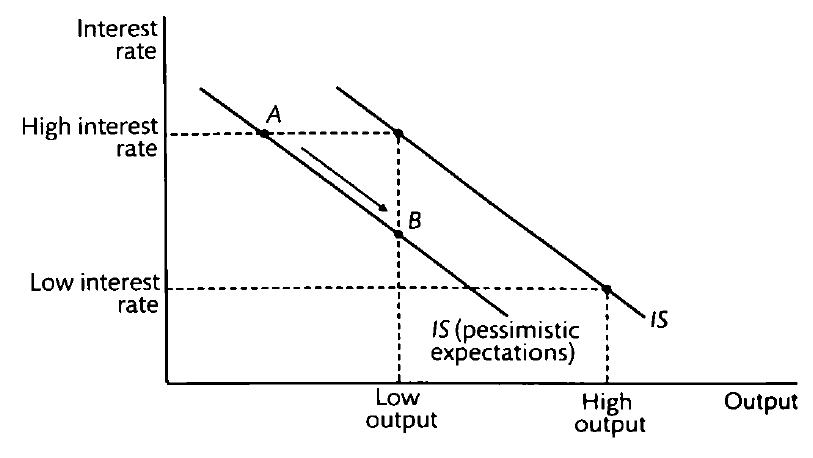
\includegraphics[width=0.8\textwidth]{./figures/aula6_fig1.PNG}
        \caption{Curva IS - efeitos de variações no otimismo e política econômica. Fonte: Carlin e Soskice (2014).}
        \label{aula6_fig1}
    \end{figure}
\end{frame}

\begin{frame}{Introdução}
    \begin{itemize}
        \item Para compreender a inclinação negativa da curva IS, considere o cenário de taxa de juros elevada e baixo produto agregado\bigskip

        \item Quando a taxa de juros é alta, os gastos com imóveis, bens de consumo duráveis e máquinas e equipamentos serão baixos\bigskip

        \item Isso significa que a demanda agregada é baixa e um baixo nível de produto agregado irá satisfazer essa baixa demanda\bigskip

        \item Considere, agora, a combinação de juros baixo e produto agregado elevado\bigskip

        \item Nesse caso, a situação é oposta: gastos elevados em imóveis, bens de consumo duráveis e com bens de investimento irão gerar um nível alto de produto e renda para os agentes econômicos
    \end{itemize}
\end{frame}

\begin{frame}{Introdução}
    \begin{itemize}
        \item Para ver como variações nas expectativas de lucros ou crescimento da renda por parte dos agentes, incerteza e o valor dos colaterais podem ser capturadas no diagrama, mantemos a taxa de juros constante e observamos os deslocamentos da curva IS\bigskip

        \item E.g.: se há expectativas pessimistas com relação aos lucros, espera-se que firmas optem por postergar decisões de novos investimentos\bigskip

        \item O resultado seria gastos com investimento mais baixos para qualquer taxa de juros dada\bigskip

        \item A curva IS se desloca para a esquerda - Figura \ref{aula6_fig1}.
    \end{itemize}
\end{frame}

\begin{frame}{Introdução}
    \begin{itemize}
        \item Utilizando o diagrama IS, podemos ver como o Banco Central e/ou o governo podem afetar o lado da demanda na economia\bigskip

        \item Em um cenário de pessimismo por parte das firmas, o BC pode decidir reduzir a taxa de juros para estimular os gastos com investimento\bigskip

        \item Isso causa um deslocamento \hlight{ao longo da curva IS} - ponto A para ponto B\bigskip

        \item Exemplo deste cenário: Federal Reserve reduz instrumento de política monetária e manteve baixa para estimular novos investimentos após a Bolha da Internet (Dotcom bubble) em 2001\bigskip

        \item Este longo período de juros baixos estimulou investimentos em construções de novos imóveis, o que teve um papel importante na CFG 2008
    \end{itemize}
\end{frame}

\begin{frame}{Introdução}    
    \begin{figure}
        \centering
        \href{https://fred.stlouisfed.org/series/NASDAQCOM}{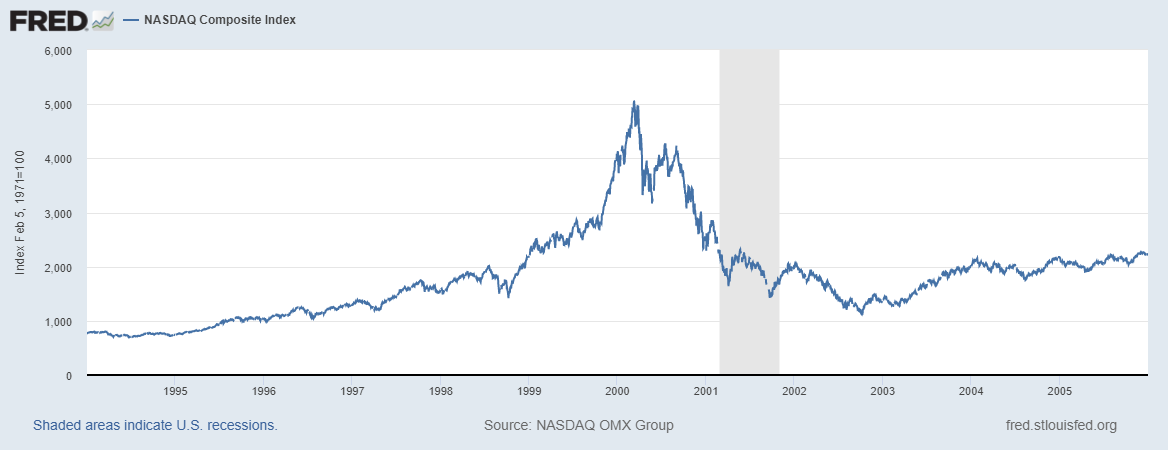
\includegraphics[width=\textwidth]{./figures/aula6_fig2.png}}
        \caption{Índice NASDAQ 1994-2005. Fonte: \href{https://fred.stlouisfed.org/series/NASDAQCOM}{Fred St. Louis}}
        \label{aula6_fig2}
    \end{figure}
\end{frame}

\begin{frame}{Introdução}
    \begin{figure}
        \centering
        \href{https://fred.stlouisfed.org/series/FEDFUNDS}{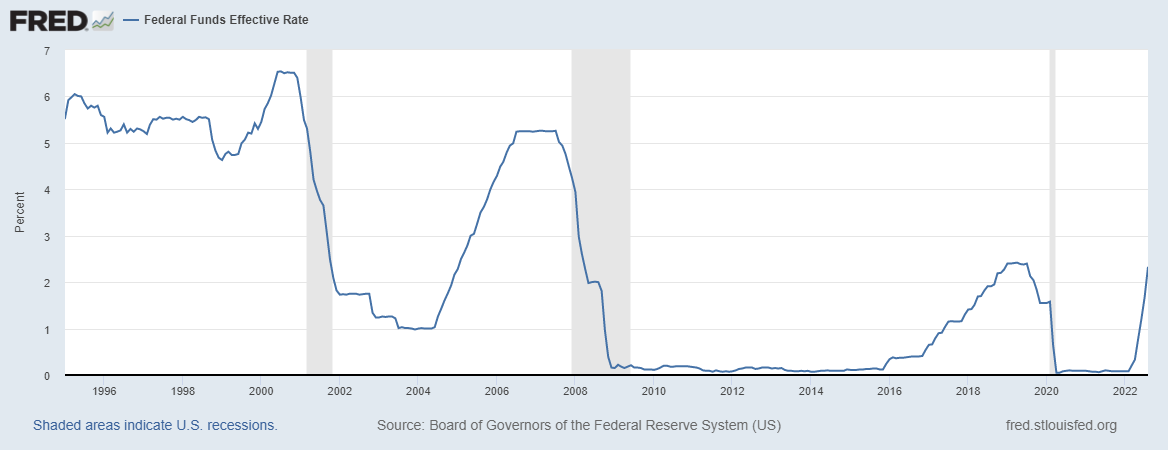
\includegraphics[width=\textwidth]{./figures/aula6_fig3.png}}
        \caption{Taxa efetiva de fundos federais. Fonte: \href{https://fred.stlouisfed.org/series/FEDFUNDS}{Fred St. Louis}.}
        \label{aula6_fig3}
    \end{figure}
\end{frame}

\begin{frame}{Introdução}
    \begin{itemize}
        \item Outra resposta possível ao deslocamento da IS para a esquerda devido às expectativas pessimistas por parte das firmas pode ser uma ação tomada pelo governo, ao invés da considerada pelo BC\bigskip

        \item Se o governo decide lançar um programa de expansão fiscal, isso deslocará a curva IS para a direita\bigskip

        \item Para cada dada taxa de juros, o governo adquire uma quantidade maior de bens e serviços\bigskip

        \item Sob nossa hipótese de que os ofertantes irão responder a essa demanda mais elevada, a economia se move para um novo ponto com nível mais elevado de produto e emprego agregados - IS se desloca para a direita, de volta para situação inicial
    \end{itemize}
\end{frame}

\begin{frame}{Introdução}
    \begin{itemize}
        \item Uma questão central em macro é qual o tamanho da expansão que um programa de gastos públicos irá gerar sobre o produto agregado\bigskip

        \item A expansão fiscal irá aumentar o produto em uma proporção de um pra um? Maior? Menor?\bigskip

        \item Como vimos nas aulas anteriores, este debate está relacionado à ideia do tamanho do \hlight{multiplicador}, i.e., qual o impacto que um aumento de 1 unidade monetária nos gastos irá ter sobre o PIB?\bigskip

        \item No diagrama IS, quanto maior o multiplicador:\bigskip

        \begin{enumerate}
            \item maior o deslocamento para a direita da curva IS associado a qualquer nível de gastos do governo adicionais\medskip

            \item menos inclinada será a curva IS, dado que com um multiplicador maior, uma redução na taxa de juros tem um efeito maior sobre o produto
        \end{enumerate}
    \end{itemize}
\end{frame}

\section{Curva IS}
\subsection{Derivação da curva IS}
\begin{frame}{Curva IS: derivação}\label{voltar}
    \begin{itemize}
        \item Ao longo deste curso, a curva IS representará o lado da demanda na economia\bigskip

        \item Objetivo, agora, é derivar a curva IS e usá-la como um ponto inicial em nossa discussão a respeito do funcionamento das políticas fiscal e monetária\bigskip

        \item \hlight{A curva IS mostra as combinações de taxa de juros real e produto agregado que equilibram o mercado de bens e serviços}\bigskip

        \item Portanto, inicialmente consideraremos a forma pela qual taxa de juros \textcolor{blue}{real} e taxa \textcolor{red}{nominal} estão relacionadas - \hyperlink{ap1}{\beamerbutton{Equação de Fisher}}:
        \begin{equation}
            r = i - \pi^e.
            \label{aula6_eq1}
        \end{equation}
    \end{itemize}
\end{frame}

\begin{frame}{Curva IS: derivação}
    \begin{itemize}
        \item Equação (\ref{aula6_eq1}): taxa de juros real é, simplesmente, a taxa nominal ajustada pela expectativa de inflação\bigskip

        \item É a taxa real de juros a mais importante para as decisões de gastos com investimento e poupança, pois representa o custo real de empréstimos (e, portanto, o retorno real sobre a poupança)\bigskip

        \item Esta taxa, então, será usada na equação de determinação do investimento e na curva IS\bigskip

        \item Quando o BC determina a taxa nominal de juros, o faz com a intenção de conseguir atingir uma taxa de juros real particular, dado que tem por objetivo influenciar os gastos que são sensíveis à variações na taxa de juros
    \end{itemize}
\end{frame}

\begin{frame}{Curva IS: derivação}
    \begin{itemize}
        \item Neste curso, assumiremos que existe apenas uma taxa de juros na economia que se aplica para todos os empréstimos e poupanças\bigskip

        \item Essa hipótese é feita para manter a matemática o mais simples possível\bigskip

        \item No entanto, no ``mundo real'', existe todo um espectro de taxas de juros\bigskip

        \item E.g., a taxa de juros sobre empréstimos bancários é tipicamente mais elevada que a taxa determinada pelo BC\bigskip

        \item Além disso, as taxas de juros diferem para títulos de diferentes maturidades\bigskip

        \item Questões relacionadas ao \emph{mark-up} bancário e a diferença entre taxas de juros de curto e longo prazo não serão tratadas
    \end{itemize}
\end{frame}

\begin{frame}{Curva IS: derivação}
    \begin{figure}
        \centering
        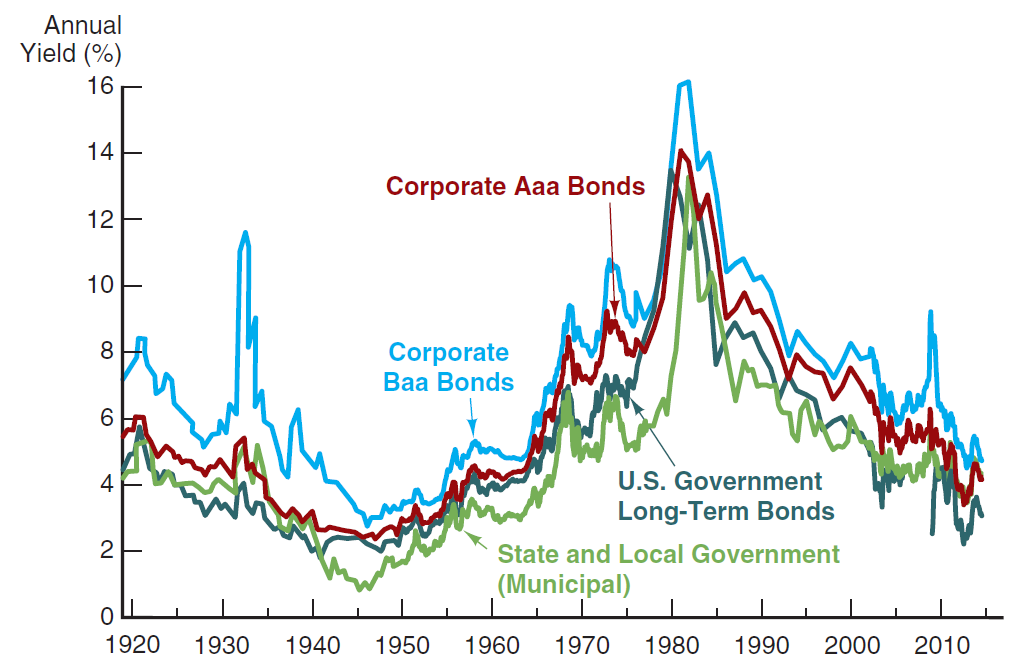
\includegraphics[width=0.7\textwidth]{./figures/aula6_fig4.PNG}
        \caption{Retorno de títulos de longo prazo, EUA - 1919-2014. Fonte: Mishkin (2016).}
        \label{aula6_fig4}
    \end{figure}
\end{frame}

\begin{frame}{Curva IS: derivação}
    \begin{figure}
        \centering
        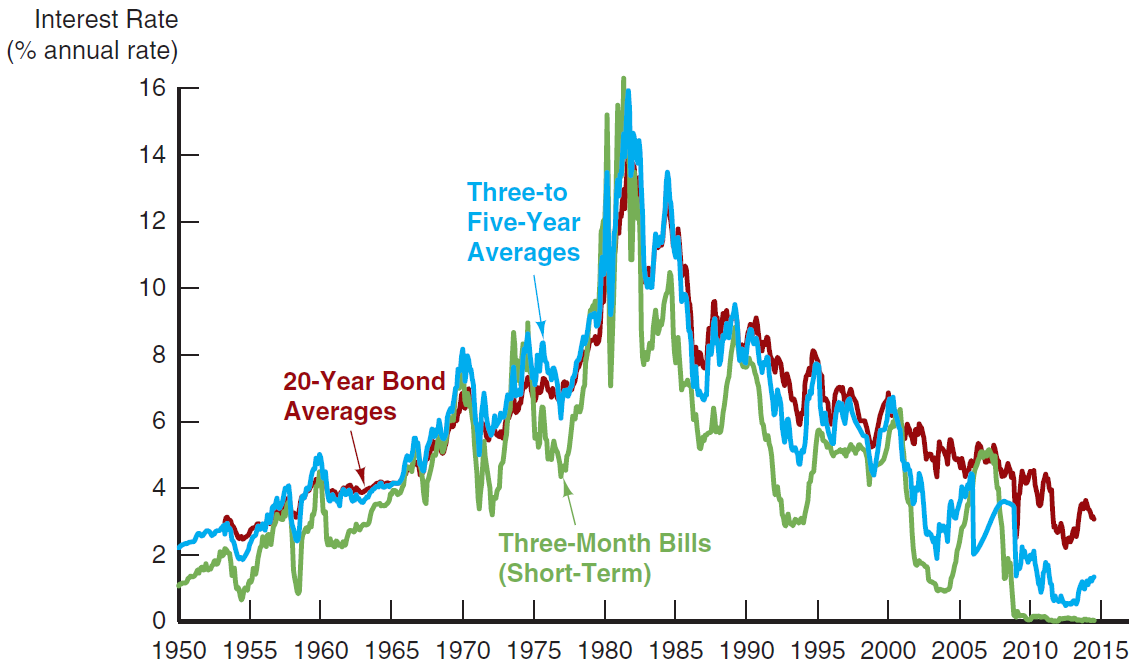
\includegraphics[width=0.7\textwidth]{./figures/aula6_fig5.PNG}
        \caption{Movimentos ao longo do tempo da taxa de juros de títulos do governo dos EUA com diferentes maturidades. Fonte: Mishkin (2016).}
        \label{aula6_fig5}
    \end{figure}
\end{frame}

\begin{frame}{Curva IS: derivação}
    \begin{itemize}
        \item Assumiremos que decisões de consumo independem da taxa de juros - hipótese que relaxaremos mais a frente\bigskip

        \item Isso significa que a \textcolor{purple}{transmissão da política monetária} operará via seu efeito sobre os gastos com investimento\bigskip

        \item Nas aulas anteriores, assumimos que o investimento era determinado pela expectativa de lucros futuros - variável que consideramos exógena\bigskip

        \item Agora incorporaremos a taxa de juros na função investimento:
        \begin{equation}
            I = a_0 - a_1 r,
            \label{aula6_eq2}
        \end{equation}
        onde $r$ é a taxa real de juros, $a_0, a_1$ são constantes e $a_1 > 0$\bigskip

        \item O principal determinante dos gastos com investimento é a expectativa de lucros futuros (pós-taxação), capturado pelo termo $a_0$
    \end{itemize}
\end{frame}

\begin{frame}{Curva IS: derivação}
    \begin{itemize}
        \item Podemos, então, obter uma relação entre a taxa de juros real e o produto agregado real, que é a curva IS:
        \begin{eqnarray}
            Y &=& \frac{1}{1-c_1(1-\tau)}[c_0 + (a_0 - a_1r) + G], \label{aula6_eq3} \\
            &=& \kappa [c_0 + (a_0 - a_1r) + G], \nonumber \\
            &=& \kappa(c_0 + a_0 + G) - \kappa a_1 r. \nonumber
        \end{eqnarray}        
        
        \item Portanto, a curva IS é dada por:
        \begin{equation}
            Y = A - ar, \label{aula6_eq4}
        \end{equation}
        onde $A \equiv \kappa(c_0 + a_0 + G)$ e $a \equiv \kappa a_1$
    \end{itemize}
\end{frame}

\begin{frame}{Curva IS: derivação}
    \begin{itemize}
        \item A derivação da curva IS evidencia o fato que, dado $r$, o produto de equilíbrio é obtido ao multiplicarmos consumo e investimento autônomos e gastos do governo pelo multiplicador $\kappa$\bigskip

        \item Isso nos dá uma combinação de juros reais e produto agregado no plano $r \times Y$ na curva IS\bigskip

        \item Fica evidente que um multiplicador mais elevado, $\uparrow\kappa$, ou uma agenda de investimentos mais elástica, $\uparrow a_1$, aumenta o efeito de uma variação na taxa de juros real sobre o produto agregado, tornando a curva IS mais plana
    \end{itemize}
\end{frame}

\begin{frame}{Curva IS: derivação}
    \begin{figure}
        \centering
        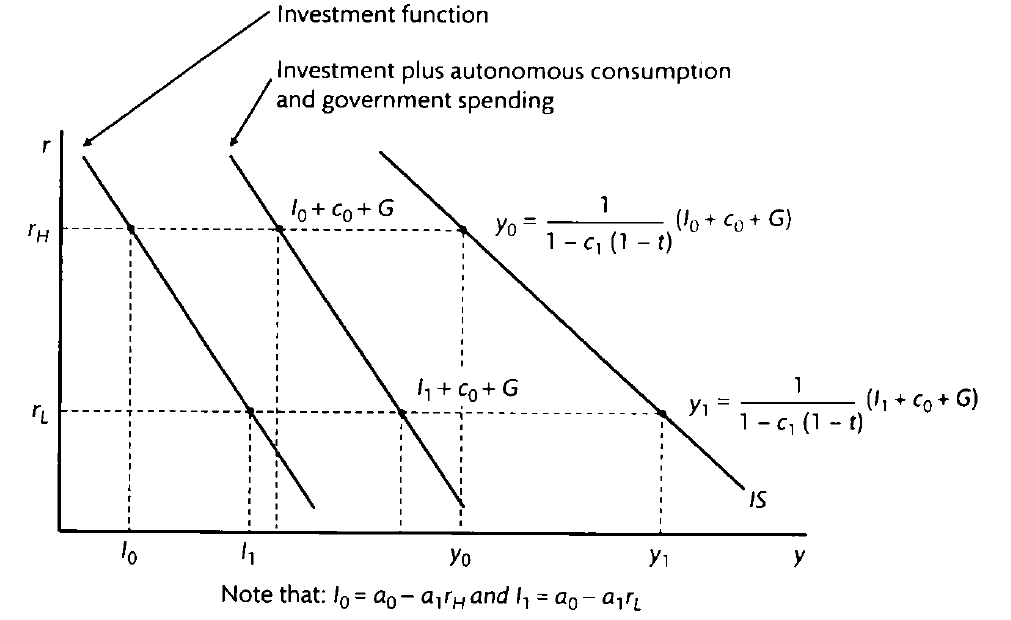
\includegraphics[width=0.7\textwidth]{./figures/aula6_fig6.PNG}
        \caption{Derivação da curva IS. Fonte: Carlin e Soskice (2014)}
        \label{aula6_fig6}
    \end{figure}
\end{frame}

\begin{frame}{Curva IS: derivação}
    \begin{itemize}
        \item A curva IS é derivada graficamente na Figura \ref{aula6_fig6}\bigskip

        \item Pela equação (\ref{aula6_eq4}) e diagrama \ref{aula6_fig6}, podemos resumir as propriedades da curva IS da seguinte maneira:\bigskip

        \begin{enumerate}
            \item Curva IS é negativemente inclinada\medskip

            \item Inclinação da curva IS:\medskip

            \begin{itemize}
                \item Variações no multiplicador alteram a inclinação. Aumentos na propensão marginal a consumir, $\uparrow c_1$, ou reduções na alíquota de imposto, $\downarrow \tau$, aumentam o multiplicador, tornando IS menos inclinada\medskip

                \item Variações na elasticidade-juros do investimento, $a_1$, alteram a inclinação. Investimentos mais sensíveis a variações nos juros, $\uparrow a_1$, levam a IS menos inclinada
            \end{itemize}
            \item Variações no consumo autônomo, investimento autônomo ou gastos do governo ($c_0, a_0, G$) deslocam a curva IS em uma magnitude dada pela variação no gasto autônomo multiplicada pelo multiplicador
        \end{enumerate}
    \end{itemize}
\end{frame}

\section{Apêndice: Equação de Fisher}\label{ap1}
\begin{frame}{Equação de Fisher}
    \begin{itemize}
        \item Jan/1981, a taxa do T-bill com vencimento de um ano nos EUA era de 10,9\%\bigskip

        \item Jan/2006, essa mesma taxa era de apenas 4,2\%\bigskip

        \item Tomar empréstimo era claramente mais barato em 2006 do que em 1981?\bigskip

        \item Jan/1980, a inflação esperada era em torno de 9,5\%, enquanto em jan/2006 era de cerca de 2,6\%\bigskip

        \item A taxa de juros nos diz quantas unidades monetárias teremos de pagar no futuro para ter uma unidade monetária adicional no presente - mas o que consumimos são bens
    \end{itemize}
\end{frame}

\begin{frame}{Equação de Fisher}
    \begin{itemize}
        \item Quando tomamos um empréstimo, o que realmente queremos saber é de quantos bens teremos que abrir mão no futuro em trocar dos bens que obtemos no presente\bigskip

        \item Da mesma forma, quando concedemos um empréstimo, queremos saber quantos bens teremos no futuro pelos bens que abrimos mão no presente\bigskip

        \item O nível de inflação torna essa distinção importante. Qual o sentido de receber pagamentos de juros altos no futuro se a inflação for tão elevada que, com o que recebermos, não conseguimos adquirir mais bens?
    \end{itemize}
\end{frame}

\begin{frame}{Equação de Fisher}
    \begin{itemize}
        \item \hlight{Taxas de juros nominais} são as taxas de juros expressas em unidades monetárias: se a taxa nominal de juros é $i_t$, tomar emprestado \$1 neste ano exigirá que se pague $1 + i_t$ unidades monetárias no próximo ano\bigskip

        \item \hlight{Taxas de juros reais} são as taxas de juros expressas em termos de uma cesta de bens: se a taxa real de juros é $r_t$, tomar emprestado o equivalente a uma cesta de bens neste ano exige que se pague o equivalente a $1 + r_t$ cestas de bens no próximo ano\bigskip
    \end{itemize}
\end{frame}

\begin{frame}{Equação de Fisher}
    \begin{itemize}
        \item Qual a relação entre as \textcolor{purple}{taxas de juros nominais} e \textcolor{blue}{taxas de juros reais} (normalmente não observáveis)?\bigskip

        \item Se tomarmos um empréstimo suficiente para adquirir uma cesta de bens neste ano, a uma taxa de juros nominal $i_t$, quanto teremos de pagar, em termos de cestas de bens, no próximo ano?\bigskip

        \item Seja $P_t$ o índice de preços ao consumidor (IPC), para adquirir uma cesta de bens hoje devemos tomar emprestado $P_t$ e pagar $(1 + i_t)P_t$ no próximo ano\bigskip

        \item Se a expectativa do nível de preços no próximo ano é $P_{t+1}^e$, o montante que se espera pagar no próximo ano é, portanto: $(1 + i_t)P_t/P_{t+1}^e$
    \end{itemize}
\end{frame}

\begin{frame}{Equação de Fisher}
    \begin{itemize}
        \item Portanto, a \textcolor{blue}{taxa de juros real} de um ano, $r_t$, é dada por:
        \begin{equation}
            1 + r_t = (1 + i_t)\frac{P_t}{P_{t+1}^e}.
            \label{aula6_ap_eq1}
        \end{equation}
        
        \item A \textcolor{blue}{taxa de inflação esperada} entre $t$ e $t+1$ é definida como:
        \begin{equation}
            \pi_{t+1}^e \equiv \frac{P_{t+1}^e - P_t}{P_t}.
            \label{aula6_ap_eq2}
        \end{equation}
        
        \item Portanto:
        \begin{equation}
            1 + r_t = \frac{1 + i_t}{1 + \pi_{t+1}^e}.
            \label{aula6_ap_eq3}
        \end{equation}
    \end{itemize}
\end{frame}

\begin{frame}{Equação de Fisher}
    \begin{itemize}
        \item A equação (\ref{aula6_ap_eq3}) nos dá a relação \textbf{exata} entre taxa de juros real, taxa de juros nominal e expectativa de inflação\bigskip

        \item Se a taxa de juros nominal e a inflação esperada não forem muito elevadas - e.g., menos de 20\% ao ano - podemos aproximar essa equação da seguinte forma:
        \begin{equation}
            r_t \approx i_t - \pi_{t+1}^e.
            \label{aula6_ap_eq4}
        \end{equation}
        
        \begin{enumerate}
            \item Quando a inflação esperada é igual a zero, as taxas de juros nominal e real são iguais\medskip

            \item Visto que a inflação esperada normalmente é positiva, a taxa de juros real é normalmente mais baixa que a taxa nominal\medskip

            \item Para uma dada taxa de juros nominal, quanto maior a expectativa inflacionária, menor a taxa de juros real
        \end{enumerate}
    \end{itemize}
\end{frame}

\begin{frame}{Equação de Fisher}
    \begin{figure}
        \centering
        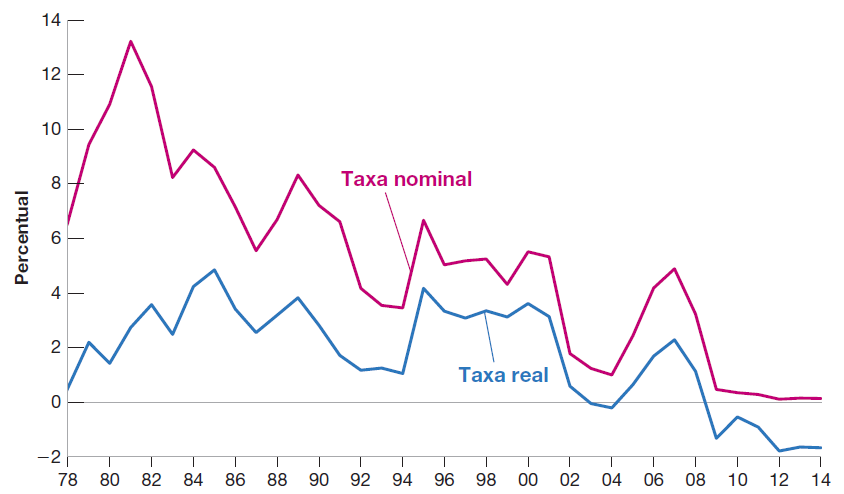
\includegraphics[width=0.7\textwidth]{./figures/aula6_fig7.PNG}
        \caption{Taxas de juros nominal e real de T-bill com vencimento em um ano nos EUA desde 1978. Fonte: Blanchard (2017)}
        \label{aula6_ap_fig1}
    \end{figure}
\end{frame}

\begin{frame}{Equação de Fisher}
    \begin{itemize}
        \item Mencionamos, anteriormente, que a taxa de juros nominal em jan/2006 era consideravelmente menor que em jan/1981\bigskip
        \item Para respondermos à questão se tomar empréstimos era mais barato em 2006 que em 1981, precisamos olhar para a taxa de juros real\bigskip

        \item A Figura \ref{aula6_ap_fig1} mostra a importância do ajuste para a inflação\bigskip

        \item Embora a taxa de juros nominal tenha sido muito menor em 2006 que em 1981, a taxa de juros real foi mais elevada nesse período\bigskip

        \item A taxa de juros real foi de cerca de 1,7\% em 2006 e 1,4\% em 1981\bigskip

        \item Dito de outra forma, apesar do acentuado declínio nas taxas de juros nominais, tomar crédito custou efetivamente mais caro em 2006 do que em 1981\bigskip

        \item Isso porque a inflação, durante este período, baixou continuamente (e com ela a expectativa de inflação)
    \end{itemize}
\end{frame}

\begin{frame}{Equação de Fisher}
    \begin{itemize}
        \item Portanto, \textcolor{purple}{as expectativas inflacionárias irão determinar a divergência entre taxas real e nominal de juros}\bigskip

        \item Deve-se mencionar que apenas um destes três termos é observável: a taxa nominal de juros, $i$\bigskip

        \item A taxa real de juros pode ser estimada a partir dos dados históricos de taxa nominal de juros e taxa de inflação - \textcolor{purple}{taxa de juros real \emph{ex-post}}\bigskip

        \item Alternativamente, uma medida \textcolor{blue}{\emph{ex-ante}} pode ser derivada em um modelo que é capaz de predizer a inflação\bigskip

        \item Por fim, se um país emite títulos que são protegidos com relação à inflação - valor de face indexado pela taxa de inflação - então, o retorno deste título é uma taxa de juros real e pode fornecer uma terceira medida\bigskip

        \item Em países centrais, são poucos os que emitem títulos indexados à inflação (UK 1981, EUA 1997, França 1998) \hyperlink{voltar}{\beamerbutton{Voltar}}
    \end{itemize}
\end{frame}

\begin{frame}{\emoji{books} Bibliografia}
    \begin{itemize}
        \item BLANCHARD, O. Macroeconomia. 7.ed. São Paulo: Pearson Education do Brasil, 2017\medskip        
        \item CARLIN, W.; SOSKICE, D. Macroeconomics: Institutions, instability, and the financial system. Oxford, UK: Oxford University Press, 2015\medskip
        \item DORNBUSCH, R.; FISCHER, S.; STARTZ, R. Macroeconomia. 11.ed. Porto Alegre: AMGH, 2013. Disponível em: \href{https://app.minhabiblioteca.com.br/books/9788580551853}{app.minhabiblioteca.com.br/books/9788580551853}\medskip
        \item MISHKIN, F.S. The economics of money, banking, and financial markets. 11.ed. Pearson Education Limited, England, 2016.
    \end{itemize}
\end{frame}
\end{document}